\documentclass[10pt,openany]{article}
\usepackage{ctex} 
\usepackage{geometry,graphicx,xcolor,color}
\geometry{
	a4paper,
	top=25.4mm, bottom=25.4mm,
	left=20mm, right=20mm,
	headheight=2.17cm,
	headsep=4mm,
	footskip=12mm
}
\usepackage[all,pdf]{xy}
\usepackage{amssymb,amsmath,mathrsfs}             
\usepackage{mathpazo}
\usepackage[nofontspec]{newpxtext}
\usepackage{array}
\usepackage{amsmath}
\usepackage{amssymb}
\usepackage{enumerate}
\usepackage{amsthm}
\usepackage{bm}
\usepackage{mathtools}
\usepackage{mathrsfs}
\usepackage{tcolorbox}
\usepackage{indentfirst}
\usepackage{setspace}
\usepackage{subfigure} 
\usepackage{tkz-fct}
\usetikzlibrary{calc,intersections,through,backgrounds,3d}
\usepackage{tkz-euclide}
\usepackage{pgfplots}
\usepackage{booktabs}
\usepackage{float}
\usepackage[graphicx]{realboxes}
\usepackage{fancyhdr}

\definecolor{winered}{rgb}{0.5,0,0}
\definecolor{structurecolor}{RGB}{122,122,142}
\definecolor{main}{HTML}{3D445F}
\definecolor{second}{HTML}{627581}
\definecolor{third}{HTML}{333333}
\definecolor{deepgreen}{HTML}{2F5E4E}  
\definecolor{purple}{HTML}{512E5F}   

\usepackage{hyperref}
\hypersetup{colorlinks = true, linktoc=all, linkcolor=blue, urlcolor=winered}


\usepackage{amsthm}
% 设定颜色(假设你在别处定义了 \color{main} 等)
\usepackage{xcolor}
\usepackage{etoolbox}
% 定义定理风格
\usepackage{amsthm}
\newtheoremstyle{defstyle}
{0.3cm}{0.3cm}{\fangsong}{-1cm}{\bfseries\color{main}}{}{0.5em}
{\indent 【\thmname{#1} \thmnumber{#2}】\ifthenelse{\equal{#3}{}}{}{~\thmnote{(#3)}}}

\newtheoremstyle{thmstyle}
{0.3cm}{0.3cm}{\kaishu}{-1cm}{\bfseries\color{second}}{}{0.5em}
{\indent 【\thmname{#1} \thmnumber{#2}】\ifthenelse{\equal{#3}{}}{}{~\thmnote{(#3)}}}

\newtheoremstyle{remstyle}
{0.3cm}{0.3cm}{\kaishu}{-1cm}{\bfseries\color{third}}{}{0.5em}
{\indent 【\thmname{#1} \thmnumber{#2}】\ifthenelse{\equal{#3}{}}{}{~\thmnote{(#3)}}}

\newtheoremstyle{exastyle}
{0.3cm}{0.3cm}{\kaishu}{-1cm}{\bfseries\color{deepgreen}}{}{0.5em}
{\indent 【\thmname{#1} \thmnumber{#2}】\ifthenelse{\equal{#3}{}}{}{~\thmnote{(#3)}}}

\newtheoremstyle{prostyle}
{0.3cm}{0.3cm}{\kaishu}{-1cm}{\bfseries\color{purple}}{}{0.5em}
{\indent 【\thmname{#1} \thmnumber{#2}】\ifthenelse{\equal{#3}{}}{}{~\thmnote{(#3)}}}

\theoremstyle{thmstyle} %theorem style
\newtheorem{theorem}{定理}[subsection]
\theoremstyle{defstyle} % definition style
\newtheorem{definition}[theorem]{定义}
\newtheorem{lemma}[theorem]{引理}
\newtheorem{corollary}[theorem]{推论}
\theoremstyle{prostyle} % proposition style
\newtheorem{proposition}[theorem]{命题}
\newtheorem{property}[theorem]{性质}
\theoremstyle{exastyle} 
\newtheorem{example}[theorem]{例}
\AtEndEnvironment{example}{\hfill \( \diamondsuit \)}
\theoremstyle{remstyle} 
\newtheorem{remark}[theorem]{注}

\renewenvironment{proof}[1][证明]{\par\underline{\textbf{#1.}} \;\fangsong}{\qed\par}
\newenvironment{solution}{\par\underline{\textbf{解.}} \;\fangsong}{\qed\par}
\newcommand{\intro}[1]{\rightline{\parbox[t]{5cm}{\footnotesize \fangsong\quad\quad #1 }}}

\AtEndEnvironment{proof}{\vspace{1.5ex}}
\AtEndEnvironment{solution}{\vspace{1.5ex}}

\usepackage{titlesec, titletoc}
\linespread{1.2} 				
\usepackage{fancyhdr}
\fancyhf{}
\renewcommand{\headrule}{\color{structurecolor}\hrule width\textwidth}
\pagestyle{fancy}
\renewcommand{\headrulewidth}{1pt}
\fancypagestyle{plain}{\renewcommand{\headrulewidth}{0pt}\fancyhf{}\renewcommand{\headrule}{}}

\fancyhead[c]{\color{structurecolor}\kaishu\rightmark}
\fancyfoot[c]{\color{structurecolor}\small\thepage}


\titleformat{\section}[frame]{\normalfont\color{structurecolor}}{\footnotesize \enspace \large \textcolor{structurecolor}{\S \,\thesection}\enspace}{6pt}{\Large\filcenter \bf \kaishu }


\titleformat{\subsection}[hang]{\bfseries}{\large\bfseries\color{structurecolor}\thesubsection\enspace}{1pt}{\color{structurecolor}\large\bfseries\filright}

\titleformat{\subsubsection}[hang]{\bfseries}{\large\bfseries\color{structurecolor}\thesubsubsection\enspace}{1pt}{\color{structurecolor}\large\bfseries\filright}

\usepackage{titling}
\renewcommand*{\maketitle}{
	\begin{titlepage}
		\newgeometry{margin = 0in}
		\parindent=0pt
		\includegraphics[width=\linewidth]{cover.png}
		\vfill
		\begin{center}
			\parbox{0.618\textwidth}{
				\hfill {\bfseries \Huge \thetitle} \\[0.6pt]  
				\rule{0.618\textwidth}{4pt} \\ 
			}
		\end{center}
		\vfill
		\begin{center}
			\parbox{0.618\textwidth}{
				\hfill\Large
				\kaishu 
				\begin{tabular}{r|}
					\textbf{2025 Summer} \\
					作者:\theauthor \\ 
					时间:\thedate \\
				\end{tabular}
			}
		\end{center}
		\vfill
		\begin{center}
			\parbox[t]{0.7\textwidth}{\centering \kaishu}
		\end{center}
		\vfill
	\end{titlepage}
	\restoregeometry
	\thispagestyle{empty}
}

\newcommand{\T}{^{\text{T}}}
\newcommand{\Her}{^{\text{H}}}
\newcommand{\F}{\mathbb{F}}
\newcommand{\gf}{\text{GL}_n(\mathbb{F})}
\newcommand{\C}{\mathbb{C}}
\newcommand{\R}{\mathbb{R}}
\newcommand{\Q}{\mathbb{Q}}
\newcommand{\n}{^{n \times n}}
\newcommand{\mn}{^{m \times n}}
\newcommand{\nm}{^{n \times m}}
\newcommand{\tz}{\mathrm{char} \;}
\newcommand{\tr}{\mathrm{tr}}
\newcommand{\diag}{\mathrm{diag}}
\newcommand{\oneb}{\underline{\hspace{1em}}\hspace{0.001em}}
\newcommand{\twob}{\oneb\oneb}
\newcommand{\fourb}{\twob\twob}
\newcommand{\tenb}{\twob\twob\twob\twob\twob}
\newcommand{\tideparallel}{%  
	\mathrel{%  
		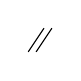
\begin{tikzpicture}[scale=0.2, baseline={([yshift=-0.5ex]current bounding box.center)}]  
			\draw[thin] (0,0) -- (1,1.5);  
			\draw[thin] (0.5,0) -- (1.5,1.5);  
		\end{tikzpicture}%  
	}%  
}  
\newcommand{\fourch}[4]
{\\[3pt]
	\begin{tabular}
		{*{4}{@{}p{4cm}}}
		A.~#1 & B.~#2 & C.~#3 & D.~#4
	\end{tabular}	
}
\newcommand{\fourchh}[4]
{\\[5pt]
	\begin{tabular}
		{*{4}{@{}p{20cm}}}
		A.~#1 \\[5pt] B.~#2 \\[5pt] C.~#3 \\[5pt] D.~#4
	\end{tabular}	
}
\newcommand{\fourchhh}[4]
{\\[3pt]
	\begin{tabular}
		{*{4}{@{}p{7.5cm}}}
		A.~#1 & B.~#2 \\[2pt] C.~#3 & D.~#4
	\end{tabular}	
}
\newcommand{\independent}{\perp\!\!\!\perp}
\everymath{\displaystyle}
\allowdisplaybreaks




\begin{document}

\pagestyle{fancy}
\lhead{Lecture 2}
\chead{illusion \& FzRainD}
\rhead{\today}

\setcounter{section}{1}
\section{可逆矩阵和行列式}

进入 \S 2 节,我们本节的任务主要是延续上节的讨论,探寻对方阵而言,什么样的方阵能在 \( \F\n \) 中可逆. 进一步,如果 \( A \) 可逆,那么解线性方程组 \( AX=\beta \) 就变得非常容易了,只需要 \( X=A^{-1}AX=A^{-1}\beta \). 我们离这种 \( n \) 个方程组成的关于 \( n \) 个变元的线性方程组的公式解,只有一步之遥,那就是如何给出 \( A^{-1} \) 的表达式?
但这些假设的前提是,我们已经知道矩阵 \( A \) 可逆,当务之急应该是找出一个判定 \( A \) 可逆的法则. 

\subsection{可逆矩阵和一般线性群}
\begin{definition}[可逆矩阵]
	设 \( A \in \F\n \),称 \( A \) 是可逆矩阵,若存在 \( B \in \F\n \) 使得 \( AB=BA=E_n \). 此时,一般记 \( B=A^{-1} \). 从定义可见,可逆矩阵与矩阵本身互为逆矩阵,即 \( A^{-1} \) 的逆矩阵也为 \( A \).
	\label{2.1.1}
\end{definition}

\begin{property}[可逆矩阵的性质]
	若矩阵 \( A, B \in \F\n \) 可逆,那么
	\begin{enumerate}[(1)]
		\item 矩阵 \( A \) 的逆元 \( B=A^{-1} \) 必定唯一;
		\item (穿脱法则 I) \ 矩阵 \( AB \) 也可逆,其逆元 \( (AB)^{-1}=B^{-1}A^{-1} \);
		\item (穿脱法则 II) \ 对一列方阵 \( \{A_k\}_{1 \leq k \leq n} \) 为可逆矩阵,那么 \( A_1A_2\cdots A_n \) 也可逆,且 \( (A_1A_2\cdots A_n)^{-1}=A_n^{-1}A_{n-1}^{-1}\cdots A_1^{-1} \);
		\item (转置与取逆的协调) \ \( A\T \) 也可逆,且 \( (A\T)^{-1}=(A^{-1})\T \).
	\end{enumerate}
	\label{2.1.2}
\end{property}

\begin{proof}
	(1) 设还有 \( C \in \F\n \) 使得 \( AC=CA=E_n \). 那么 \( C=E_nC=(BA)C=B(AC)=BE_n=B \). (2) 只需要验证定义,\( (B^{-1}A^{-1})(AB)=B^{-1}(A^{-1}A)B=B^{-1}E_nB=B^{-1}B=E_n \). 另一方面,\( (AB)(B^{-1}A^{-1})=E_n \) 是类似的. (3) 完全等同 (2),只需要用归纳法. (4) 验证 \( (A^{-1})\T(A\T)=(AA^{-1})\T=E_n\T=E_n \). 同理 \( (A\T)(A^{-1})\T= E_n \).
\end{proof}

\begin{example}[初等矩阵]
	初等矩阵均可逆. 且它们的逆矩阵十分容易求出. 可以自行验证如下的结论:
	\[ E(i,j(c))^{-1}=E(i,j(-c)), \; E(i(c))^{-1}=E(i(c^{-1})) \ (c \neq 0), \; E(i,j)^{-1}=E(i,j). \]
	现在我们明白了,所谓初等矩阵对应操作的逆操作,无非就是左乘初等矩阵的逆矩阵.
	\label{2.1.3}
\end{example}

\begin{example}[单位矩阵]
	单位矩阵显然可逆,且 \( E_n^{-1}=E_n \).
\end{example}

\begin{example}
	若矩阵 \( A,B \) 可逆,那么 \( A+B \) 不一定可逆,例如取 \( A=E_n, \; B=-E_n \),那么 \( A+B=O \). 而必定不存在矩阵 \( C \in \F\n \) 使得 \( CO=OC=E_n \)!
	\label{2.1.5}
\end{example}

事实上,在性质 \ref{2.1.2} 的证明中我们只用到了矩阵乘法的结合律,矩阵乘法存在幺元,以及可逆矩阵的定义,即定义 \ref{2.1.1}. 这提示我们性质 \ref{2.1.2} 应该具有一般性. 接下来,我们将矩阵环 \( \F\n \) 的乘法部分作如下提炼,就得到群的定义.

\begin{definition}[群]
	设 \( G \) 是一个非空集合,其上存在一个二元运算 \( \cdot: G \times G \to G \),满足
	\begin{enumerate}
		\item[(1)] \textbf{结合律} \( (ab)c=a(bc) \);
	\end{enumerate}
	那么称 \( (G,\cdot) \) 为一个半群,进一步,如果还有
	\begin{enumerate}
		\item[(2)] \textbf{幺元性质} 存在 \( e \in G \) 使得 \( ae=ea=a \);
	\end{enumerate}
	那么称 \( (G,\cdot) \) 为一个幺半群. 进一步,如果还有
	\begin{enumerate}
		\item[(3)] \textbf{存在逆元} 对 \( a \in G \),存在 \( a^{-1} \in G \) 使得 \( a(a^{-1})=(a^{-1})a=e \);
	\end{enumerate}
	\textbf{那么称 \( (G,\cdot) \) 为一个群. } 进一步,如果还有
	\begin{enumerate}
		\item[(4)] \textbf{交换律} \( ab=ba \).
	\end{enumerate}
	那么称 \( (G,\cdot) \) 为一个交换群或者 Abel 群. 上述定义中,\( a,b,c \in G \) 都是任取的.
\end{definition}

上述定义我们一点都不陌生,我们可以很清楚地发现,环和域的定义几乎完全就是满足上述定义的两种运算的拼接,并额外满足两种运算的协调性而已. 轻而易举地获得下面的例子.

\begin{example}
	设 \( \F \) 是域,那么 \( (\F,+) \) 在数的通常加法下为一个 Abel 群,记 \( \F^*:=\F \textbackslash \{0\} \),那么 \( (\F,\cdot) \) 在数的通常乘法下为一个 Abel 群. 
\end{example}

\begin{example}
	设 \( \F\n \) 是域 \( \F \) 上的全矩阵环,那么 \( (\F\n,+) \) 在通常矩阵的加法下为一个 Abel 群. 
\end{example}

\begin{example}
	记 \( \gf:=\{ A \in \F\n \mid \exists \ B \in \F\n, \; AB=BA=E_n \} \),也就是 \( \F\n \) 中的可逆矩阵全体. 那么 \( (\gf,\cdot) \) 在配备通常矩阵的乘法下为一个群,但是由于对于 \( n \geq 2 \),矩阵乘法一般不具备交换律,那么是一个非 Abel 群. 当 \( n=1 \) 时,显然 \( \text{GL}_1(\mathbb{F})= \F^* \),那么 \( (\text{GL}_1(\mathbb{F}),\cdot) \) 为一个 Abel 群. 
	
	一般称 \( (\gf,\cdot) \) 为域 \( \F \) 上的 \( n \) 级一般线性群. 注意 \( (\gf,+) \) 不是一个群,因为例 \ref{2.1.5} 告诉我们可逆矩阵全体对加法不封闭,因此不构成二元运算.
\end{example}

\begin{property}[群的性质]
	设 \( (G,\cdot) \) 为群,任取 \( a,b \in G \),那么
	\begin{enumerate}
		\item \( e \in G \) 唯一,即群中幺元唯一;
		\item \( a^{-1} \in G \) 唯一,即群中任意元素的可逆元唯一;
		\item (穿脱法则 I) \( (ab)^{-1}=b^{-1}a^{-1} \);
		\item (穿脱法则 II) 任取 \( a_1,\cdots,a_n \in G \),那么 \( (a_1a_2\cdots a_n)^{-1}=a_n^{-1}a_{n-1}^{-1}\cdots a_1^{-1} \).
	\end{enumerate}
\end{property}

\begin{proof}
	\( (2)-(4) \) 直接照搬性质 \ref{2.1.2} 的证明即可,对 \( (1) \) 注意到如存在 \( e_1 \neq e_2 \in G \) 为幺元,那么 \( e_1,e_2 \) 均为 \( e_1 \) 的幺元,而幺元唯一.
\end{proof}

下面的命题说明了可逆矩阵只能在方阵中定义,而无法推广到一般的矩阵. 

\begin{proposition}
	对 \( n \neq m \),不存在 \( A \in \F\nm \) 以及 \( B \in \F\mn \) 使得 \( AB= E_n, \; BA=E_m \).
	\label{2.1.11}
\end{proposition}

\begin{proof}
	(\textbf{法一}) \ 利用迹的性质即可,注意到若结论不然,那么 \(\tr(AB)=n \neq m=\tr(BA) \).
	
	\vspace{1ex}
	
	(\textbf{法二}) \ 不妨设 \( m>n \). 若结论不然,断言线性方程组 \( AX=O \) 只有零解. 首先 \( X=O \) 显然为解. 其次,对任意满足方程的 \( X_1 \in \F^m \) 使得 \( AX_1=O \leadsto X_1=BAX_1=BO=O \). 设 \( PA\T=K \),其中 \( P \) 为若干 \( m \) 阶矩阵的乘积,对 \( A\T \) 施行初等行变换,使其变为简化行阶梯形矩阵 \( K \). 那么非零行数目 \( r(A\T) \leq \min\{n,m\}=n<m \). 故 \( PA\T=K \) 的第 \( m \) 行必定为零行. 即 \( \varepsilon_m^T K= O_{1 \times n}= \varepsilon_m^T PA\T \). 两边同时取转置,有 \( A(P\T\varepsilon_m)=O_{n \times 1} \). 故只能 \( P\T\varepsilon_m=O \). 利用性质 \ref{2.1.2} (3),初等矩阵都为可逆矩阵,故若干初等矩阵的积也为可逆矩阵,那么由性质 \ref{2.1.2} (4) 可知 \( P\T \) 可逆,对  \( P\T\varepsilon_m=O \) 两边同乘 \( P\T \) 的逆得到 \( \varepsilon_m=O \) 矛盾.
\end{proof}

为了进一步研究可逆矩阵的判定条件,我们先对可逆矩阵有一个初步刻画.

\begin{proposition}[可逆的必要条件]
	设 \( A \in \gf \),即定义 \ref{2.1.1},存在矩阵 \( B \in \F\n \),使得 \( BA=AB=E_n \),其中 \( B \) 当然也是可逆的. 那么
	\begin{enumerate}[(1)]
		\item 线性方程组 \( AX=O \) 仅有零解;
		\item \( A \) 的简化行阶梯形矩阵为 \( E_n \) 或者简化行阶梯形矩阵的非零行数目 \( r(A)=n \);
		\item \( A \) 可以只经过初等行变换或者初等列变换变为 \( E_n \);
		\item \( A \) 可以表示为初等矩阵的乘积.
	\end{enumerate}
	\label{2.1.12}
\end{proposition}

\begin{proof}
	(1) 首先 \( X=O \) 显然为解. 其次,对每个满足线性方程组 \( AX=O \) 的解都有 \( X=A^{-1}AX=A^{-1}O=O \);
	(2) 否则,设 \( A \) 的简化行阶梯矩阵为 \( K=PA \),其中 \( P \) 为若干初等矩阵之积,为可逆矩阵. 设 \( K \) 的非零行数目 \( r(A)<n \). 即 \( \varepsilon_n\T K=O= \varepsilon_n\T PA \),那么 \( A\T(P\T \varepsilon_n)=O \). 然而由性质 \ref{2.1.2} (4) \( P\T \) 可逆,这意味着 \( P\T \varepsilon_n \neq O \). 那么 \( A\T X=O \) 存在非零解,但 \( A\T \) 可逆,矛盾. (1)(2) 事实上完全是命题 \ref{2.1.11} 法二过程的照搬.
	
	\vspace{1ex}
	
    (3) 只经过初等行变换是显然的,对初等列变换,考察 \( A\T \),由于 \( A\T \) 可以只经过初等行变换化为 \( E_n \),这就对应 \( A \) 可以只经过初等列变换化为 \( E_n \). (4) 由 (3) 立即得到.
\end{proof}

\begin{corollary}
	设 \( A \in \F\n \),那么 \( A \in \gf \) 的充分必要条件为 \( A \) 可以表示为初等矩阵的乘积.
	\label{2.1.13}
\end{corollary}

\begin{proof}
	用命题 \ref{2.1.12} 和例 \ref{2.1.3} 即可.
\end{proof}

\subsection{代数动机: 线性方程组的公式解}

\subsubsection{行列式的归纳定义}
为了研究可逆矩阵的判定条件,不妨假设 \( A \) 可逆,那么我们从 \( AX=\beta \) 的解的表达式开始研究,因为我们知道此时 \( X=A^{-1}\beta \) 就是解的表达式. 其中必定会有一些和 \( A^{-1} \) 有关的量. 从二元线性方程组开始,考察
\[ \left\{ \begin{array}{l}
	a_{11}x_1+a_{12}x_2=b_1, \\
	a_{21}x_1+a_{22}x_2=b_2.
\end{array}\right. \leadsto \overline{A}=\begin{bmatrix}
 a_{11} & a_{12} & b_1 \\
 a_{21} & a_{22} & b_2
\end{bmatrix}. \]

由命题 \ref{2.1.12} (2),对 \( \overline{A} \) 实行 Guass-Jordan 消元法必定能得到两个主元,不妨考虑简单情形,也就是适当调整 \( A \) 使得操作过程无须涉及行的互换变换. 在这个假定下,\( a_{11} \neq 0 \),也就是不考虑 \( a_{11}=0, a_{21} \neq 0 \),然后将第 2 行换到第 1 行. 那么
\[ \begin{bmatrix}
	a_{11} & a_{12} & b_1 \\
	a_{21} & a_{22} & b_2
\end{bmatrix} \leadsto \begin{bmatrix}
1 & a_{12}/a_{11} & b_1/a_{11} \\
a_{21} & a_{22} & b_2
\end{bmatrix} \leadsto \begin{bmatrix}
1 & \frac{a_{12}}{a_{11}} & \frac{b_1}{a_{11}} \\[2ex]
0 & a_{22} - \frac{a_{21} a_{12}}{a_{11}} & b_2 - \frac{a_{21} b_1}{a_{11}}
\end{bmatrix}. \]

此时必定有 \( a_{22}a_{11} \neq a_{21} a_{12} \),否则对 \( A \) 实行初等行变换得不到两个主元,与可逆前提矛盾. 那么
\[ \begin{bmatrix}
	1 & \frac{a_{12}}{a_{11}} & \frac{b_1}{a_{11}} \\[2ex]
	0 & a_{22} - \frac{a_{21} a_{12}}{a_{11}} & b_2 - \frac{a_{21} b_1}{a_{11}}
\end{bmatrix} \leadsto \begin{bmatrix}
1 & \frac{a_{12}}{a_{11}} & \frac{b_1}{a_{11}} \\[2ex]
0 & a_{22}a_{11} - a_{21} a_{12} & a_{11} b_2 - a_{21} b_1
\end{bmatrix} \leadsto \begin{bmatrix}
1 & \frac{a_{12}}{a_{11}} & \frac{b_1}{a_{11}} \\[2ex]
0 & 1 & \frac{a_{11} b_2 - a_{21} b_1}{a_{22}a_{11} - a_{21} a_{12}}
\end{bmatrix}. \]

进一步变为简化行阶梯形矩阵
\[ \begin{bmatrix}
	1 & \frac{a_{12}}{a_{11}} & \frac{b_1}{a_{11}} \\[2ex]
	0 & 1 & \frac{a_{11} b_2 - a_{21} b_1}{a_{22}a_{11} - a_{21} a_{12}}
\end{bmatrix} \to \begin{bmatrix}
1 & 0 & \frac{a_{12} b_2 - a_{22} b_1}{a_{22}a_{11} - a_{21} a_{12}} \\[2ex]
0 & 1 & \frac{a_{11} b_2 - a_{21} b_1}{a_{22}a_{11} - a_{21} a_{12}}
\end{bmatrix}. \]

引入记号
\[ \det A=\begin{vmatrix}
	a_{11} & a_{12} \\ a_{21} & a_{22}
\end{vmatrix}:= a_{11}a_{22}-a_{12}a_{21}=a_{11}\cdot (-1)^{1+1}a_{12}+a_{21} \cdot (-1)^{1+2}a_{12}. \]

那么上述方程的解即
\[ x_1=\frac{\begin{vmatrix}
		b_1 & a_{12} \\ b_2 & a_{22}
\end{vmatrix}}{\begin{vmatrix}
		a_{11} & a_{12} \\ a_{21} & a_{22}
\end{vmatrix}}, \; x_2=\frac{\begin{vmatrix}
a_{11} & b_1 \\ a_{12} & b_2
\end{vmatrix}}{\begin{vmatrix}
a_{11} & a_{12} \\ a_{21} & a_{22}
\end{vmatrix}}. \]

显然为了使得上述表达式成立,在操作过程我们用到了 \( \det A \neq 0 \). 而对于解的分子,都是和 \( \beta \) 的信息混合在一起,难以提取有关 \( A^{-1} \) 存在的必要信息. 但这只给出了一个大概方向,如何定义更高阶矩阵 \( A \) 的 \(  \det A \) 呢? 进一步,如果定义好了 \( \det A \) 并且发现 \( \det A \neq 0 \),真的能推出矩阵可逆吗? 为了找到一个合适的定义,接着考察三元线性方程组,

\[ \left\{ \begin{array}{l}
	a_{11}x_1+a_{12}x_2+a_{13}x_3=b_1, \\
	a_{21}x_1+a_{22}x_2+a_{23}x_3=b_2, \\
	a_{31}x_1+a_{32}x_2+a_{33}x_3=b_3.
\end{array}\right. \leadsto \overline{A}=\begin{bmatrix}
	a_{11} & a_{12} & a_{13} & b_1 \\
	a_{21} & a_{22} & a_{23} & b_2 \\
	a_{31} & a_{32} & a_{33} & b_3 
\end{bmatrix}. \]

一开始仍然不妨设 \( a_{11} \neq 0 \),那么
\[ \overline{A} \leadsto  \begin{bmatrix}
	1 & a_{12}/a_{11} & a_{13}/a_{11} & b_1/a_{11} \\[2ex]
	0 & a_{22}-\frac{a_{21}a_{12}}{a_{11}} & a_{23}-\frac{a_{21}a_{13}}{a_{11}} & b_2-\frac{b_1a_{12}}{a_{11}} \\[2ex]
	0 & a_{32}-\frac{a_{31}a_{12}}{a_{11}} & a_{33}-\frac{a_{31}a_{13}}{a_{11}} & b_3-\frac{b_1a_{12}}{a_{11}}
\end{bmatrix} \leadsto \begin{bmatrix}
1 & a_{12}/a_{11} & a_{13}/a_{11} & b_1/a_{11} \\[2ex]
0 & a_{22} a_{11} - a_{21} a_{12} & a_{23} a_{11} - a_{21} a_{13} & b_2 a_{11} - b_1 a_{21} \\[2ex]
0 & a_{32} a_{11} - a_{31} a_{12} & a_{33} a_{11} - a_{31} a_{13} & b_3 a_{11} - b_1 a_{31}
\end{bmatrix}. \]

那么子矩阵
\[ \begin{bmatrix}
	a_{22} a_{11} - a_{21} a_{12} & a_{23} a_{11} - a_{21} a_{13} & b_2 a_{11} - b_1 a_{21} \\[2ex]
	 a_{32} a_{11} - a_{31} a_{12} & a_{33} a_{11} - a_{31} a_{13} & b_3 a_{11} - b_1 a_{31}
\end{bmatrix} \]

的简化行阶梯矩阵具有两个主元,将其看成二元线性方程组,由前述,得到解的表达式
\[ x_2=\frac{\begin{vmatrix}
		b_2 a_{11} - b_1 a_{21} & a_{23} a_{11} - a_{21} a_{13} \\ b_3 a_{11} - b_1 a_{31} & a_{33} a_{11} - a_{31} a_{13}
\end{vmatrix}}{\begin{vmatrix}
		a_{22} a_{11} - a_{21} a_{12} & a_{23} a_{11} - a_{21} a_{13} \\ a_{32} a_{11} - a_{31} a_{12} & a_{33} a_{11} - a_{31} a_{13}
\end{vmatrix}}, \; x_3=\frac{\begin{vmatrix}
		a_{22} a_{11} - a_{21} a_{12} & b_2 a_{11} - b_1 a_{21} \\ a_{32} a_{11} - a_{31} a_{12} & b_3 a_{11} - b_1 a_{31}
\end{vmatrix}}{\begin{vmatrix}
a_{22} a_{11} - a_{21} a_{12} & a_{23} a_{11} - a_{21} a_{13} \\ a_{32} a_{11} - a_{31} a_{12} & a_{33} a_{11} - a_{31} a_{13}
\end{vmatrix}}. \]

先化简上式的分母,得到
\begin{align*}
	& \quad \begin{vmatrix}
		a_{11} {\color{teal} a_{22}} - a_{21} {\color{violet} a_{12}} & a_{23} a_{11} - a_{21} a_{13} \\
		{\color{cyan!40!black} a_{32}} a_{11} - a_{31} {\color{violet} a_{12}} & a_{33} a_{11} - a_{31} a_{13}
	\end{vmatrix} \\[1ex]
	&= ({\color{teal} a_{22}} a_{11} - a_{21} {\color{violet} a_{12}})(a_{33} a_{11} - a_{31} a_{13}) - (a_{23} a_{11} - a_{21} a_{13})({\color{cyan!40!black} a_{32}} a_{11} - a_{31} {\color{violet} a_{12}}) \\[1ex]
	&= a_{11}(\, a_{11} a_{33} {\color{teal} a_{22}}- a_{11} {\color{cyan!40!black} a_{32}} a_{23}  + a_{21} a_{13} {\color{cyan!40!black} a_{32}} - a_{21} {\color{violet} a_{12}} a_{33} + a_{31} a_{23} {\color{violet} a_{12}} - a_{31} a_{13}  {\color{teal} a_{22}}   \,) \\[1ex]
	&= a_{11} \left( a_{11} \begin{vmatrix}
{\color{teal} a_{22}} & a_{23} \\
{\color{cyan!40!black} a_{32}} & a_{33}
	\end{vmatrix}
	- a_{21} \begin{vmatrix}
		{\color{violet} a_{12}} & a_{13} \\
		{\color{cyan!40!black} a_{32}} & a_{33} 
	\end{vmatrix}
	+ a_{31} \begin{vmatrix}
		{\color{violet} a_{12}} & a_{13} \\
		{\color{teal} a_{22}} & a_{23} 
	\end{vmatrix} \right)
\end{align*}

类似化简 \( x_2 \) 的分子,
\begin{align*}
	& \quad \begin{vmatrix}
		{\color{teal} b_2} a_{11} - {\color{violet} b_1} a_{21} & a_{23} a_{11} - a_{21} a_{13} \\
		{\color{cyan!40!black} b_3} a_{11} - {\color{violet} b_1} a_{31} & a_{33} a_{11} - a_{31} a_{13}
	\end{vmatrix} \\[1ex]
	&= ({\color{teal} b_2} a_{11} - {\color{violet} b_1} a_{21})(a_{33} a_{11} - a_{31} a_{13}) - ({\color{cyan!40!black} b_3} a_{11} - {\color{violet} b_1} a_{31})({\color{cyan!40!black} a_{32}} a_{11} - a_{31} {\color{violet} a_{12}}) \\[1ex]
	&= a_{11}(\, a_{11} a_{33} {\color{teal} b_2}- a_{11} {\color{cyan!40!black} b_{3}} a_{23}  + a_{21} a_{13} {\color{cyan!40!black} b_{3}} - a_{21} {\color{violet} b_{1}} a_{33} + a_{31} a_{23} {\color{violet} b_{1}} - a_{31} a_{13}  {\color{teal} b_{2}} \,) \\[1ex]
	&= a_{11} \left( a_{11} \begin{vmatrix}
		{\color{teal} b_{2}} & a_{23} \\
		{\color{cyan!40!black} b_{3}} & a_{33}
	\end{vmatrix}
	- a_{21} \begin{vmatrix}
		{\color{violet} b_{1}} & a_{13} \\
		{\color{cyan!40!black} b_{3}} & a_{33} 
	\end{vmatrix}
	+ a_{31} \begin{vmatrix}
		{\color{violet} b_{1}} & a_{13} \\
		{\color{teal} b_{2}} & a_{23} 
	\end{vmatrix} \right)
\end{align*}

注意观察,我们对分子其实无需展开计算,只需要进行替换 \( {\color{violet} a_{12} \leadsto b_1}, \; {\color{teal} a_{22} \leadsto b_2}, \; {\color{cyan!40!black} a_{23} \leadsto b_3} \) 即可. 这事实上就是我们在本节最后叙述的 Cramer 法则. 定义

\begin{align*}
	\det A &=\begin{vmatrix}
		a_{11} & a_{12} & a_{13} \\
		a_{21} & a_{22} & a_{23} \\
		a_{31} & a_{32} & a_{33} 
	\end{vmatrix}:=a_{11} \begin{vmatrix}
		a_{22} & a_{23} \\
		a_{32} & a_{33}
	\end{vmatrix}
	- a_{21} \begin{vmatrix}
		a_{12} & a_{13} \\
		a_{32} & a_{33} 
	\end{vmatrix}
	+ a_{31} \begin{vmatrix}
		a_{12} & a_{13} \\
		a_{22} & a_{23} 
	\end{vmatrix} \\
	&= (-1)^{1+1}a_{11} \begin{vmatrix}
		a_{22} & a_{23} \\
		a_{32} & a_{33}
	\end{vmatrix}
	+(-1)^{2+1} a_{21} \begin{vmatrix}
		a_{12} & a_{13} \\
		a_{32} & a_{33} 
	\end{vmatrix}
	+(-1)^{3+1}a_{31} \begin{vmatrix}
		a_{12} & a_{13} \\
		a_{22} & a_{23} 
	\end{vmatrix}
\end{align*}


那么
\[ x_2= \frac{\begin{vmatrix}
		a_{11} & b_1 & a_{13} \\
		a_{21} & b_2 & a_{23} \\
		a_{31} & b_3 & a_{33} 
\end{vmatrix}}{\begin{vmatrix}
		a_{11} & a_{12} & a_{13} \\
		a_{21} & a_{22} & a_{23} \\
		a_{31} & a_{32} & a_{33} 
\end{vmatrix}}, \; x_3=\frac{\begin{vmatrix}
a_{11} & a_{12} & b_1 \\
a_{21} & a_{22} & b_2 \\
a_{31} & a_{32} & b_3 
\end{vmatrix}}{\begin{vmatrix}
a_{11} & a_{12} & a_{13} \\
a_{21} & a_{22} & a_{23} \\
a_{31} & a_{32} & a_{33} 
\end{vmatrix}}. \]

带回 \( x_1+(a_{12}/a_{11})x_2+(a_{13}/a_{11}) x_3=b_1/a_{11} \),经过计算可以得到类似的结果,即
\[ x_1=\frac{\begin{vmatrix}
		b_{1} & a_{12} & a_{13} \\
		b_{2} & a_{22} & a_{23} \\
		b_{3} & a_{32} & a_{33} 
\end{vmatrix}}{\begin{vmatrix}
		a_{11} & a_{12} & a_{13} \\
		a_{21} & a_{22} & a_{23} \\
		a_{31} & a_{32} & a_{33} 
\end{vmatrix}}. \]

于是我们下面提出行列式的第一种定义,按列展开的数学归纳法定义.

\begin{definition}[数学归纳法定义]
	考虑 \( A \in \F\n \),现在递归定义 \( \det A \ (|A|): \F\n \to \F \). 当 \( n=1 \) 时,设 \( A=(a) \),定义 \( \det A=a \). 现在假设 \( n-1 \) 阶的行列式已经定义好,设元素 \( a_{ij} \) 的余子式为从 \( A \) 中删去第 \( i \) 行和第 \( j \) 列所得 \( n-1 \) 阶矩阵的行列式,记作 \( M_{ij} \),即
	\[ M_{ij}=\det \begin{bmatrix}
		a_{11} & \cdots & a_{1,j-1} & a_{1,j+1} & \cdots & a_{1n} \\
		\vdots &        & \vdots   & \vdots   &        & \vdots \\
		a_{i-1,1} & \cdots & a_{i-1,j-1} & a_{i-1,j+1} & \cdots & a_{i-1,n} \\
		a_{i+1,1} & \cdots & a_{i+1,j-1} & a_{i+1,j+1} & \cdots & a_{i+1,n} \\
		\vdots &        & \vdots   & \vdots   &        & \vdots \\
		a_{n1} & \cdots & a_{n,j-1} & a_{n,j+1} & \cdots & a_{nn}
	\end{bmatrix}. \]
	
	记元素 \( a_{ij} \) 的代数余子式为 \( A_{ij}:=(-1)^{i+j}M_{ij} \).那么 \( \det A=|A|:= a_{11}A_{11}+a_{21}A_{21}+\cdots+a_{n1}A_{n1} \). 这一定义称为按第一列展开归纳定义.
	\label{2.2.1}
\end{definition}

\subsubsection{行列式的基本性质}

这个定义是否有用,还需要看它能不能用来解决我们先前的问题: 即可逆矩阵的判定以及线性方程组的公式解. 那么沿着定义,我们第一步自然是刻画一些相关的性质.

\begin{property}[行列式的性质]
	在定义 \ref{2.2.1} 的基础上,将矩阵按列分块,得到 \( A=(\alpha_1,\alpha_2,\cdots,\alpha_n) \),也记行列式 \( \det A=\det(\alpha_1,\alpha_2,\cdots,\alpha_n) \). 任取 \( \beta \in \F^n \) 以及 \( c \in \F \),那么
	\begin{enumerate}[(1)]
		\item 将 \( \det A \) 的一列乘以某个常数 \( c \) 得到 \( \det B \),那么 \( \det B=c\det A \). 即 \( \det(\alpha_1,\cdots,\alpha_{i-1},c\alpha_i,\alpha_{i+1},\cdots,\alpha_n)=c\det A \),进而 \( \det(cA)=c^n \det A \);
		\item 一般没有 \( \det(A+B)=\det A+\det B \),但是有 \( \det(\alpha_1,\cdots,\alpha_{i-1},\alpha_i+\beta,\alpha_{i+1},\cdots,\alpha_n)=\det(\alpha_1,\alpha_2,\cdots,\alpha_n)+\det(\alpha_1,\cdots,\alpha_{i-1},\beta,\alpha_{i+1},\cdots,\alpha_n) \);
		\item 交换行列式的两列,行列式改变符号,即 \( \det(\cdots,\alpha_{i-1},\alpha_j,\alpha_{i+1},\cdots,\alpha_{j-1},\alpha_i,\alpha_{j+1},\cdots)=-\det A \ (i<j) \).
	    \item 对矩阵 \( A \) 的列作倍法变换,行列式的值不变. 即将行列式的一列乘以常数 \( c \) 加到另一列上,行列式的值不变.
	    \[ \det(\cdots,\alpha_{i-1},\alpha_i+c\alpha_j,\alpha_{i+1},\cdots,\alpha_{j-1},\alpha_j,\alpha_{j+1},\cdots)=\det A. \]
	    \item \( \det A \) 可以按第 \( r \ (1\leq r \leq n) \) 列展开,即
	    \[ \det A= a_{1r}A_{1r}+a_{2r}A_{2r}+\cdots+a_{nr}A_{nr}. \]
	    \item 转置不改变行列式的值,即 \( \det A\T= \det A \).
	\end{enumerate}
	\label{2.2.2}
\end{property}

\begin{proof}
     (1)(2) 用归纳法是非常容易的. 现考虑 (3). 用数学归纳法,若交换的是非第一列的两列即证. 现在考虑若交换的是第一列和第二列的情况,设 \( A \) 经过该交换得到矩阵 \( B \). 记矩阵 \( A,B \) 的余子式为 \( M_{ij}, \; N_{ij} \). 自然有 \( M_{i2}=N_{i1} \). 将 \( \det B \) 按第一列展开
     \[ \det B= \sum_{i=1}^{n} (-1)^{i+1} b_{i1}N_{i1}= \sum_{i=1}^{n} (-1)^{i+1} a_{i2}M_{i2}= -\sum_{i=1}^{n} (-1)^{i+2} a_{i2}M_{i2}. \]
     
     现在只要证明 \( \det A \) 能按第二列展开即可. 设矩阵 \( A \) 删去第 \( i,k \) 行以及 \( 1,2 \) 列余下矩阵的行列式为 \( M\begin{bmatrix}
     i & k \\ 1 & 2
     \end{bmatrix} \).
     
     利用定义 \ref{2.2.1} 有
     \begin{align*}
     	\det A & = \sum_{i=1}^{n} (-1)^{i+1}a_{i1}M_{i1} \\
     	&= \sum_{i=1}^{n} (-1)^{i+1}a_{i1} \left(\sum_{k=1}^{i-1}a_{k2}(-1)^{k+1}M\begin{bmatrix}
     		i & k \\ 1 & 2
     	\end{bmatrix}+\sum_{k=i+1}^{n}a_{k2}(-1)^{(k-1)+1}M\begin{bmatrix}
     	i & k \\ 1 & 2
     	\end{bmatrix} \right) \\
     	&= \sum_{1 \leq k<i \leq n}^{} (-1)^{i+k} a_{i1}a_{k2} \begin{bmatrix}
     		i & k \\ 1 & 2
     	\end{bmatrix}+ \sum_{1 \leq i<k \leq n}^{}  (-1)^{i+k+1} a_{i1}a_{k2} \begin{bmatrix}
     	i & k \\ 1 & 2
     	\end{bmatrix} \\
     	&= \sum_{k=1}^{n} (-1)^{k+2}a_{k2} \left( \sum_{i=k+1}^{n} (-1)^{i-1+1}a_{i1}M\begin{bmatrix}
     		i & k \\ 1 & 2
     	\end{bmatrix}+ \sum_{i=1}^{k-1}(-1)^{i+1}a_{i1}M\begin{bmatrix}
     	i & k \\ 1 & 2
     	\end{bmatrix} \right) \\
     	&= \sum_{k=1}^{n} (-1)^{k+2}a_{k2}M_{k2}.
     \end{align*}
     
     现在我们已经证明了结论对第 1, 2 列互换以及不含第一列的互换成立. 对第 1, \( k \) 列互换的情形,记 \( (i,j) \) 为第 \( (i,j) \) 列互换的操作,\( (i_2,j_2)(i_1,j_1) \) 这样的复合表示先互换 \( i_1,j_1 \) 列,再互换 \( i_2,j_2 \) 列. 那么 \( (1,k)=(k-1,k)\cdots(3,4)(2,3)(1,2)(2,3)(3,4)\cdots(k-1,k) \). 上述每一次互换都改变一次行列式的符号,一共进行了 \( 2(k-1)+1 \) 次互换,行列式的值自然改变符号.
     
     推论 \ref{2.2.3} 直接来源于 (3). 利用推论 \ref{2.2.3} 以及 (2),又可以得到 (4). (5) 的证明只需要对行列式作互换 \( (1,2)(2,3)(3,4)\cdots(r-1,r) \),然后按第一列展开即可. 为证明 (6),我们先断言若行列式的一行全为零,那么行列式为零,利用归纳假设即得. 然后说明 \( \det A \) 可以按第一行展开,反复利用 (2),
     \begin{align*}
     	\det A= \begin{vmatrix}
     		a_{11} & a_{12} & \cdots & a_{1n} \\
     		a_{21} & a_{22} & \cdots & a_{2n} \\
     		\vdots & \vdots & \ddots & \vdots \\
     		a_{n1} & a_{n2} & \cdots & a_{nn}
     	\end{vmatrix} &=  \begin{vmatrix}
     	a_{11} & a_{12} & \cdots & a_{1n} \\
     	0 & a_{22} & \cdots & a_{2n} \\
     	\vdots & \vdots & \ddots & \vdots \\
     	0 & a_{n2} & \cdots & a_{nn}
     	\end{vmatrix}+ \begin{vmatrix}
     	0 & a_{12} & \cdots & a_{1n} \\
     	a_{21} & a_{22} & \cdots & a_{2n} \\
     	\vdots & \vdots & \ddots & \vdots \\
     	a_{n1} & a_{n2} & \cdots & a_{nn} \\
     \end{vmatrix} \\
     	&= a_{11}A_{11}+\begin{vmatrix}
     		0 & a_{12} & \cdots & a_{1n} \\
     		a_{21} & a_{22} & \cdots & a_{2n} \\
     		\vdots & \vdots & \ddots & \vdots \\
     		a_{n1} & a_{n2} & \cdots & a_{nn} \\
     	\end{vmatrix} \\
     	&= a_{11}A_{11}+ \begin{vmatrix}
     	0 & a_{12} & \cdots & a_{1n} \\
     	a_{21} & 0 & \cdots & a_{2n} \\
     	\vdots & \vdots & \ddots & \vdots \\
     	a_{n1} & 0 & \cdots & a_{nn} \\
     	\end{vmatrix}+\begin{vmatrix}
     	0 & 0 & \cdots & a_{1n} \\
     	a_{21} & a_{22} & \cdots & a_{2n} \\
     	\vdots & \vdots & \ddots & \vdots \\
     	a_{n1} & a_{n2} & \cdots & a_{nn} \\
     	\end{vmatrix} \\
     	&= a_{11}A_{11}+a_{12}A_{12}+\cdots \\
     	&=  a_{11}A_{11}+a_{12}A_{12}+\cdots+a_{1n}A_{1n}+ \begin{vmatrix}
     		0 & 0 & \cdots & 0 \\
     		a_{21} & a_{22} & \cdots & a_{2n} \\
     		\vdots & \vdots & \ddots & \vdots \\
     		a_{n1} & a_{n2} & \cdots & a_{nn} \\
     	\end{vmatrix} \\
     	&= \det A+0.
     \end{align*}
     
     最后对 \( A\T \) 按第一行展开完全等同于对 \( A \) 按第一列展开,即 \( \det A=\det A\T \).
\end{proof}


\begin{corollary}
	若行列式有两列相同,那么行列式的值为 0.
	\label{2.2.3}
\end{corollary}

\begin{proof}
	若 \( \tz \F \neq 2 \),根据性质 \ref{2.2.2} (4),交换这两个相同的列,可以得到 \( \det A=-\det A \),进而 \( 2\det A=0 \) 蕴含 \( \det A=0 \).  \( \tz \F=2 \) 时,由于 \( -1=1 \),那么任意交换行列式的列,行列式的值均不变. 用数学归纳法即可,当 \( n=2 \) 时显然成立,对 \( n>2 \),将两个相同的列调换至第 \( 2 \sim n \) 列,再按第一列展开用归纳假设即可.
\end{proof}

\begin{corollary}
	利用性质 \ref{2.2.2} (7),可以直接把性质 \ref{2.2.2} 中所有有关列的表述改为行,都完全成立.
	\label{2.2.4}
\end{corollary}

\begin{corollary}
	若行列式有一行或者一列全为零,那么行列式的值为 0.
	\label{2.2.5}
\end{corollary}

\begin{proof}
	有许多证明方法,例如用性质 \ref{2.2.2} (1) 选择一个非零常数 \( c \) 乘到这一个全为零的行/列 或者性质 \ref{2.2.2} (2) 将 \( 0 \) 拆分为 \( 0+0 \),或者按全为零的列或者行展开,即性质 \ref{2.2.2} (5),还可以把其余任意一行/列加到这一个全为零的行/列,进而用推论 \ref{2.2.3}. 
\end{proof}

\subsubsection{可逆矩阵的判定和 Cramer 法则}

有了性质 \ref{2.2.2} 我们可以得出下面两个重要的命题,进而体会行列式的工具性: 刻画可逆矩阵的充要条件以及给出一类线性方程组的公式解.

\begin{definition}[伴随矩阵]
	设 \( A \in \F\n \),定义矩阵 \( A \) 的古典伴随矩阵为 \( A^*:=(A_{ji}) \),即按正常行列顺序排列 \( a_{ij} \) 的代数余子式,而后转置. 
	\label{2.2.6}
\end{definition}

\begin{proposition}[正交性]
	在定义 \ref{2.2.6} 的基础上,成立 \( AA^*=A^*A=(\det A)E_n \). 换言之,用矩阵乘法的定义就写出
	\[ a_{1i}A_{1j}+a_{2i}A_{2j}+\cdots+a_{ni}A_{nj}=(\det A)\delta_{ij}, \]
	以及
	\[ a_{i1}A_{j1}+a_{i2}A_{j2}+\cdots+a_{in}A_{jn}=(\det A)\delta_{ij}. \]
	\label{2.2.7}
\end{proposition}

\begin{proof}
	对 \( i=j \),就是性质 \ref{2.2.2} (5) 和推论 \ref{2.2.4}. 对 \( i \neq j \),不妨 \( i<j \),以第一个式子为例,构造行列式
	\[ \det \bordermatrix{
		& & i & & j &  \cr
		&\cdots & a_{1i} & \cdots & a_{1i} & \cdots \cr
		&\cdots & a_{2i} & \cdots & a_{2i} & \cdots \cr
		&\vdots & \vdots & \ddots & \vdots & \vdots \cr
		&\cdots & a_{ni} & \cdots & a_{ni} & \cdots 
	}= a_{1i}A_{1j}+a_{2i}A_{2j}+\cdots+a_{ni}A_{nj}=0. \]
	
	这里对第 \( j \) 列展开,且运用推论 \ref{2.2.3}.
\end{proof}

\begin{lemma}
	设 \( A \in \F\n, \; B \in \F^{m \times m}, \; C \in  \F\mn \),那么
	\[ \det \begin{bmatrix}
		A & O \\
		C & B
	\end{bmatrix}= \det A \det B. \]
	\label{2.2.8}
\end{lemma}

\begin{proof}
	对 \( n \) 用归纳法. 当 \( n=1 \) 时,按第一行展开立即得到. 设对 \( n-1 \) 命题成立,考虑一般的 \( n \). 为方便讨论,下面 \( M_{ij} \) 表示 \( (i,j) \) 元的余子式对应的矩阵,也表示余子式本身. 那么对原矩阵按第一行展开得到
	\begin{align*}
		\det \begin{bmatrix}
			A & O \\
			C & B
		\end{bmatrix} &= (-1)^{1+1} a_{11} \det \begin{bmatrix}
		M_{11} & O \\
		* & B
		\end{bmatrix}+ (-1)^{1+2} a_{12} \det \begin{bmatrix}
		M_{12} & O \\
		* & B
		\end{bmatrix}+\cdots+ (-1)^{1+n} a_{1n} \det \begin{bmatrix}
		M_{1n} & O \\
		* & B
		\end{bmatrix} \\
		&= \left[\sum_{i=1}^{n} (-1)^{i+1}a_{1i}M_{1i}\right] \det B= \det A \det B.
	\end{align*}
\end{proof}

\begin{proposition}[同态性]
	设 \( A,B \in \F\n \),那么 \( \det(AB)=(\det A)(\det B) \).
	\label{2.2.9}
\end{proposition}

\begin{proof}
	考虑分块矩阵
	\[  \begin{bmatrix}
		A & O \\
		-E & B
	\end{bmatrix}=\begin{bmatrix}
	a_{11} & a_{12} & \cdots & a_{1n} & 0 & 0 & \cdots & 0 \\
	a_{21} & a_{22} & \cdots & a_{2n} & 0 & 0 & \cdots & 0 \\
	\vdots & \vdots & \ddots & \vdots & \vdots & \vdots & \ddots & \vdots \\
	a_{n1} & a_{n2} & \cdots & a_{nn} & 0 & 0 & \cdots & 0 \\
	-1 & 0 & \cdots & 0  & b_{11} & b_{12} & \cdots & b_{1n} \\
    0 & -1 & \cdots & 0  & b_{21} & b_{22} & \cdots & b_{2n} \\
	\vdots & \vdots & \ddots & \vdots & \vdots & \vdots & \ddots & \vdots \\
	0 & 0 & \cdots & -1 & b_{n1} & b_{n2} & \cdots & b_{nn} 
	\end{bmatrix}. \]
	
	我们要做的无非就是用分块初等变换
	\[ \begin{bmatrix}
		A & O \\
		-E & B
	\end{bmatrix} \leadsto \begin{bmatrix}
	A-AE & O+AB \\
	-E & B
	\end{bmatrix} \]
	
	但是这不是简单的初等变换,我们知道只有倍法变换不会改变行列式,那么这样的分块初等变换能变成若干倍法变换的复合吗,试一试就知道了. 现在左乘 \( E(1,2n(a_{1n}))\cdots E(1,n+2(a_{12}))E(1,n+1(a_{11})) \),这样就能将 \( A \) 的第一行全部打成零,那么观察 \( B \) 上方矩阵的第一行,设它的 \( (1,j) \) 元为 \( c_{1j} \). 那么
	\[ c_{1j}= b_{1j}a_{11}+b_{2j}a_{12}+\cdots+b_{nj}a_{1n}=(AB)_{1j}. \]
	
	类似的方法,接下来依次干掉 \( A \) 的 \( 2\sim n \) 行,就完成了前述分块初等变换的作用,那么事实上也就得到了分块倍法变换也就是若干倍法变换的复合. 我们依旧记 \( B \) 上方矩阵的 \( (i,j) \) 元为 \( c_{ij} \). 利用倍法变换不改变行列式的值,那么
	\[ \det \begin{bmatrix}
		A & O \\
		-E & B
	\end{bmatrix}= \det \begin{bmatrix}
	 0 & 0 & \cdots & 0 & c_{11} & c_{12} & \cdots & c_{1n} \\
	 0 & 0 & \cdots & 0 & c_{21} & c_{22} & \cdots & c_{2n} \\
	\vdots & \vdots & \ddots & \vdots & \vdots & \vdots & \ddots & \vdots \\
	  0 & 0 & \cdots & 0 & c_{n1} & c_{n2} & \cdots & c_{nn} \\
	-1 & 0 & \cdots & 0  & b_{11} & b_{12} & \cdots & b_{1n} \\
	0 & -1 & \cdots & 0  & b_{21} & b_{22} & \cdots & b_{2n} \\
	\vdots & \vdots & \ddots & \vdots & \vdots & \vdots & \ddots & \vdots \\
	0 & 0 & \cdots & -1 & b_{n1} & b_{n2} & \cdots & b_{nn} 
	\end{bmatrix}. \]
	
	由引理 \ref{2.2.8},左端也就是 \( \det A \det B \). 对右端按第一列展开,发现只剩下 \( (-1)^{(n+1)+1} \cdot (-1) M_{n+1,1} \). 再对 \( M_{n+1,1} \) 按第一列展开,又只剩下 \( (-1)^{(n+1)+1} \cdot (-1) M'_{n+1,1} \). 这样不断进行下去第 \( n \) 次展开只剩下 \( (-1)^{(n+1)+1} \cdot (-1) \det (AB) \). 综合起来就有
	\[ (\det A)(\det B)=(-1)^{n(n+1)+2(1+\cdots+1)} \cdot \det (AB)= (-1)^{2n(n+1)} \det (AB)= \det(AB). \]
	
	对右端还可以进行列的对换,实行 \( (1,n+1)(2,n+2)\cdots(n,2n) \) 后,原行列式变为
	\[ \begin{bmatrix}
		c_{11} & c_{12} & \cdots & c_{1n} & 0 & 0 & \cdots & 0 \\
		c_{21} & c_{22} & \cdots & c_{2n} & 0 & 0 & \cdots & 0 \\
		\vdots & \vdots & \ddots & \vdots & \vdots & \vdots & \ddots & \vdots \\
		c_{n1} & c_{n2} & \cdots & c_{nn} & 0 & 0 & \cdots & 0 \\
		b_{11} & b_{12} & \cdots & b_{1n} & -1 & 0 & \cdots & 0 \\
		b_{21} & b_{22} & \cdots & b_{2n} & 0 & -1 & \cdots & 0 \\
		\vdots & \vdots & \ddots & \vdots & \vdots & \vdots & \ddots & \vdots \\
		b_{n1} & b_{n2} & \cdots & b_{nn} & 0 & 0 & \cdots & -1
	\end{bmatrix} \]
	
	用引理 \ref{2.2.8},就得到右端行列式的值为 \( (-1)^n \det (AB) \).
\end{proof}

\begin{remark}
	引理 \ref{2.2.8} 和命题 \ref{2.2.9} 的证明也可以使用 Laplace 定理来完成,见课本. 但是这个需要太多铺垫,本讲义不从.
\end{remark}

\begin{corollary}
	设 \( A,B \in \F\n \),那么 \( \det(AB)=\det(BA) \).
\end{corollary}

\begin{proof}
	用命题 \ref{2.2.9} 立即得到,这说明矩阵乘法交换下的不变量还有行列式.
\end{proof}

\begin{example}
	对 \( A \in \F\nm, B \in \F\mn \),未必有 \( \det(AB)=\det(BA) \)! 例如
	\[ A= \begin{bmatrix}
		1 & 2
	\end{bmatrix}, \; B=\begin{bmatrix}
	1 \\ 2
	\end{bmatrix} \leadsto \det(AB)=5 \neq 0=\det(BA). \]
	
	 另外,这时候 \( \det A \) 和 \( \det B \) 均没有定义,命题 \ref{2.2.9} 也失效了,关于这一点的推广,在本节的最后我们会讨论 Cauchy\(-\)Binet 公式.
\end{example}

有了命题 \ref{2.2.7} 和命题 \ref{2.2.9},我们现在终于可以把命题 \ref{2.1.12} 推广到充分必要条件,也就是可逆矩阵的判定.

\begin{proposition}[可逆矩阵的判定,充分必要条件]
	设 \( A \in \F\n \),那么下列叙述等价:
	\begin{enumerate}[(1)]
		\item \( A \in \gf \),即定义 \ref{2.1.1},存在矩阵 \( B \in \F\n \),使得 \( BA=AB=E_n \);
		\item \( \det A \neq 0 \);
		\item 存在矩阵 \( B \in \F\n \),使得 \( AB=E_n \) 或者 \( BA=E_n \);
		\item 线性方程组 \( AX=O \) 仅有零解;
		\item \( A \) 的简化行阶梯形矩阵为 \( E_n \) 或者简化行阶梯形矩阵的非零行数目 \( r(A)=n \);
		\item \( A \) 可以只经过初等行变换或者初等列变换变为 \( E_n \);
		\item \( A \) 可以表示为初等矩阵的乘积.
	\end{enumerate}
	\label{2.2.13}
\end{proposition}

\begin{proof}
	由推论 \ref{2.1.13},那么 \( (7) \Leftrightarrow (1) \) 已经得到.
	 
	先证明 \( (3) \Rightarrow (2) \Rightarrow (1) \Rightarrow (3) \). 若 存在矩阵 \( B \in \F\n \),使得 \( AB=E_n \),那么由命题 \ref{2.2.9} \( \det(AB)=\det A \det B=1 \neq 0 \leadsto \det A \neq 0 \). 当 \( \det A \neq 0 \),由命题 \ref{2.2.7} 得到 \( AA^*=A^*A=(\det A) E \),取 \( B=(\det A)^{-1}A^* \) 就回到 \( A \) 可逆的定义. 而 \( (1) \Rightarrow (3) \) 是显然的.
	
	由命题 \ref{2.1.12} 知道 \( (1)  \Rightarrow (4)(5)(6) \),且显然 \( (5)(6) \Rightarrow (3) \Leftrightarrow (1) \). 那么 \( (1)(5)(6) \) 的等价性也体现了. 现在说明 \( (4) \Rightarrow (6) \Leftrightarrow (1) \) 即可. 若 \( A \) 不能经过初等列变换变为 \( E_n \),那么 \( A\T \) 不能经过初等行变换变为 \( E_n \),即 \( A\T \) 的简化行阶梯矩阵非零行数目 \( r(A\T) <n \). 于是 \( \varepsilon_n\T A\T=\bm{0} \leadsto A\varepsilon_n=\bm{0} \). 导出矛盾.
\end{proof}

那么下面关于不可逆矩阵的等价刻画,简直是呼之欲出.

\begin{proposition}[不可逆矩阵的判定,充分必要条件]
	设 \( A \in \F\n \),那么下列叙述等价:
	\begin{enumerate}[(1)]
		\item \( A \) 不可逆;
		\item \( \det A = 0 \);
		\item 线性方程组 \( AX=O \) 有无穷多解;
		\item 存在非零矩阵 \( B \in \F\n \) 使得 \( AB=O \);
		\item \( A \) 的简化行阶梯形矩阵的非零行数目 \( r(A)<n \).
	\end{enumerate}
	\label{2.2.14}
\end{proposition}

\begin{proof}
	(3) 就是指 \( AX=O \) 存在非零解,那么对一个解 \( X_0 \),自然所有 \( cX_0 \ (c \in \F) \) 就都是解了. \( (3) \Rightarrow (4) \),取一个非零解 \( X_0 \),构造 \( B=(X_0,\bm{0},\cdots,\bm{0}) \) 即可. \( (4) \Rightarrow (3) \): 设 \( B=(B_1,\cdots,B_n) \),那么必定存在一个 \( B_i \neq \bm{0} \). 由于分块矩阵的乘法定义,那么 \( AB_i=O \). 其余充要性直接由命题 \ref{2.2.13} 得到.
\end{proof}

从性质 \ref{2.1.2} 以及命题 \ref{2.2.13} 的证明我们知道,如果 \( A \) 可逆,逆元必定唯一 \( A^{-1}=(\det A)^{-1} A^* \). 那么 \( AX=\beta \) 的解就完全归结到计算一些行列式,得到 \( A^* \) 和 \( \det A \),最后计算 \( X=A^{-1}\beta \) 即可. 这就是下面的 Cramer 法则,回答了我们开头提出的如何求线性方程组公式解的问题.

\begin{theorem}[Cramer]
	给定 \( A \in \F\n \) 以及 \( \beta \in \F^n \),那么线性方程组 \( AX=\beta \) 有唯一解的充分必要条件为 \( A \) 可逆,此时解为
	\[ X=\frac{A^*\beta}{\det A}. \]
	
	进一步,若 \( A=(\alpha_1,\cdots,\alpha_n) \),那么解的分量事实上可以表示为
	\[ x_i=\frac{\det(\alpha_1,\cdots,\alpha_{i-1},\beta,\alpha_{i+1},\cdots,\alpha_n)}{\det A}. \]
	
	这和我们在二元以及三元方程组解的表达式探究中所得到的结果一致.
\end{theorem}

\begin{proof}
	充分性,首先明显 \( X=(\det A)^{-1}(A^*\beta) \) 是一个解. 若存在 \( X_1 \neq X_2 \),使得 \( AX_1=AX_2=\beta \leadsto X_1-X_2 \neq \bm{0} \) 为 \( AX=O \) 的非零解,由命题 \ref{2.2.13} (4) 推出矛盾. 
	
	必要性,用反证法,若 \( A \) 不可逆,设 \( A \) 的简化行阶梯矩阵为 \( K=PA \),其中 \( P \) 可逆,为若干初等矩阵之积. 设 \( P\beta=(b_1,\cdots,b_n)\T \),且非零行数目 \( r(A)=m<n \). 那么适当取 \( b_{m+1}=1 \),其余元素为零,此时 \( KX=(b_1,\cdots,b_n)\T \) 无解. 取 \( \beta=P^{-1}(b_1,\cdots,b_n)\T \),说明此时 \( AX=\beta \) 未必有解. 另一方面,即使有解,由命题 \ref{2.2.14} (3) 知道存在 \( X_0 \neq 0 \),使得 \( AX_0=O \). 对满足方程的任意解 \( X_1 \),\( X=X_1+cX_0 \ (c \in \F) \) 都是解,解不唯一. 故必要性成立.
	
	接下来,计算分量的表达式,设 \( \beta=(b_1,\cdots,b_n)\T \). 由矩阵乘法的定义以及古典伴随矩阵的定义 \( A^*\beta \) 的第 \( i \) 行元素为
	\[ (A^*\beta)_i=\sum_{k=1}^{n} A_{ki}b_k=\det(\alpha_1,\cdots,\alpha_{i-1},\beta,\alpha_{i+1},\cdots,\alpha_n). \]
	
	最后一个等号由行列式按第 \( i \) 列展开得到,即性质 \ref{2.2.2} (5).
\end{proof}

到此为止,可以说关于本节开始之前所提出的问题,都获得了圆满的回答. 剩下的部分,则是对我们新定义的行列式提供几个例子练习,以及给出它的一种几何含义便于我们进一步理解它存在的意义.

\subsubsection{简单的行列式计算}

我们会在章节总复习时多练习一些困难的行列式,现在先来看几个基本的例子.

\begin{example}[上三角行列式]
	给定上三角矩阵
	\[ A= 
	\begin{bmatrix}
		a_{11} & a_{12} & \cdots & a_{1n} \\
		0      & a_{22} & \cdots & a_{2n} \\
		\vdots & \vdots & \ddots & \vdots \\
		0      & 0      & \cdots & a_{nn}
	\end{bmatrix}. 
	\]
	证明 \( \det A=a_{11}a_{22}\cdots a_{nn} \). 同理,如果将 \( A \) 取转置,利用性质 \ref{2.2.2} (6) 就能得到下三角行列式也等于主对角元素的乘积.
\end{example}

\begin{proof}
	从第一列开始展开即可,每次的展开式都只剩下一项,那么
	\[ \det A= (-1)^{1+1}a_{11} \cdot (-1)^{1+1}a_{22} \cdots (-1)^{1+1} a_{nn}=a_{11}a_{22}\cdots a_{nn}. \]
\end{proof}

利用 Guass-Jordan 消元法我们知道,任何一个方阵都可以经过初等行变换化为上三角矩阵 (简化行阶梯形矩阵就是上三角矩阵,对方阵而言) ,而初等变换对行列式的影响无非就是增加一个负号,或者某个倍数. 但在操作量级上只有 \( \mathcal{O}(n^3) \),然而假定读者学过行列式的组合展开式,一共是有 \( n! \) 项,利用一个数学分析中熟知的无穷大量的阶
\[ \lim\limits_{n \to \infty} \frac{n^3}{n!}=0. \leadsto n^3<<n!  \]

可见初等变换在求解行列式中也有着用武之地. 下面练习一个例子.

\begin{example}
	计算 \[ \det \begin{bmatrix}
		1 & 1 & 2 & 3 \\
		1 & 3 & 6 & 1 \\
		3 & -1 & 1 & 5 \\
		2 & -5 & 0 & 1
	\end{bmatrix}. \]
\end{example}

\begin{solution}
	利用初等变换知道
	\[ \begin{bmatrix}
		1 & 1 & 2 & 3 \\
		1 & 3 & 6 & 1 \\
		3 & -1 & 1 & 5 \\
		2 & -5 & 0 & 1
	\end{bmatrix} \leadsto \begin{bmatrix}
	1 & 1 & 2 & 3 \\
	0 & 2 & 4 & -2 \\
	0 & -4 & -5 & -4 \\
	0 & -7 & -4 & -5
	\end{bmatrix} \leadsto 2 \begin{bmatrix}
	1 & 1 & 2 & 3 \\
	0 & 1 & 2 & -1 \\
	0 & -4 & -5 & -4 \\
	0 & -7 & -4 & -5
\end{bmatrix} \leadsto 2 \begin{bmatrix}
1 & 1 & 2 & 3 \\
0 & 1 & 2 & -1 \\
0 & 0 & 3 & -8 \\
0 & 0 & 10 & -12
\end{bmatrix} \leadsto 6 \begin{bmatrix}
1 & 1 & 2 & 3 \\
0 & 1 & 2 & -1 \\
0 & 0 & 1 & -8/3 \\
0 & 0 & 0 & 44/3
\end{bmatrix}.   \]

那么最后的结果为 \( 6 \cdot 44/3=88 \). 这里的系数只是为了计算行列式的简单记法,不代表矩阵的数乘.
\end{solution}

\begin{example}[爪型行列式]
	设下述行列式的主对角元素均非零,计算
	\[ \det A= \begin{vmatrix}
		a_0 & b_1 & \cdots & b_n \\
		c_1 & a_1 &  & \\
		\vdots &  & \ddots & \\
		c_n &       &        & a_n
	\end{vmatrix}. \]
	\label{2.2.18}
\end{example}

\begin{solution}
	(\textbf{法一}) \ 利用第 \( 2 \sim n \) 列把第一列全打成零,也就是如下的初等列变换
	\[ \begin{bmatrix}
		a_0 & b_1 & \cdots & b_n \\
		c_1 & a_1 &  & \\
		\vdots &  & \ddots & \\
		c_n &       &        & a_n
	\end{bmatrix} \leadsto \begin{vmatrix}
	a_0-\frac{c_1b_1}{a_1} & b_1 & \cdots & b_n \\
	0 & a_1 &  & \\
	\vdots &  & \ddots & \\
	c_n &       &        & a_n
	\end{vmatrix} \leadsto \cdots \leadsto \begin{vmatrix}
	a_0- \sum_{i=1}^{n}\frac{c_ib_i}{a_i} & b_1 & \cdots & b_n \\
	0 & a_1 &  & \\
	\vdots &  & \ddots & \\
	0 &       &        & a_n
	\end{vmatrix}. \]
	
	这是一个上三角行列式,那么结果为 
	\[ \det A= \left( a_0- \sum_{i=1}^{n}\frac{c_ib_i}{a_i} \right) \prod_{i=1}^{n} a_i.\]
	
	(\textbf{法二}) \ 按第一行展开,先研究 \( b_i \) 对应的余子式 \( M_{1,i+1} \),容易看出它写为
	\[ M_{1,i+1}= \begin{vmatrix}
		c_1 & a_1 & & & & & \\
		\vdots & & \ddots & & & & \\
		c_{i-1} & &  & a_i & & & \\
		c_{i} & & &  &0  & & \\
		c_{i+1} & & &  & a_{i+1}  & & \\
		\vdots & & & &  & \ddots  & \\
		c_n & & & &  &  & a_n
	\end{vmatrix}\]
	
	那么再按第 \( i \) 行展开,即 \( M_{1,i+1}=(-1)^{i+1} c_i \prod_{j \neq i}^{} a_j \). 那么
	\[ \det A= \prod_{k=0}^{n} a_i- \sum_{i=1}^{n} (-1)^{i+2} b_i M_{1,i+1}= \prod_{k=0}^{n} a_i- \sum_{i=1}^{n} (-1)^{i+2} b_i \left( (-1)^{i+1} c_i \prod_{j \neq i}^{} a_j \right)= \prod_{k=0}^{n} a_i-\sum_{i=1}^{n} b_ic_i \prod_{j \neq i}^{} a_j. \]
\end{solution}

\begin{remark}
	例 \ref{2.2.18} 中当所有 \( a_i \neq 0 \) 时,法一和法二的结果必然相同,这就是组合问题中的“算两次”原理. 当存在 \( a_i =0 \) 时,法二仍然适用,而法一遗憾退场.
\end{remark}

利用例 \ref{2.2.18},我们可以计算很多种行列式,下面举出一些例子.

\begin{example}
	计算 \[
	\det A= \det \begin{bmatrix}
		x & a & a & \cdots & a \\
		a & x & a & \cdots & a \\
		a & a & x & \cdots & a \\
		\vdots & \vdots & \vdots & \ddots & \vdots \\
		a & a & a & \cdots & x
	\end{bmatrix}.
	\]
	\label{2.2.20}
\end{example}

\begin{solution}
	(\textbf{法一}) 加边法,
	\[ \det A= \det \begin{bmatrix}
		1 & a & a & a & \cdots & a \\
		0 & x & a & a & \cdots & a \\
		0 & a & x & a & \cdots & a \\
		0 & a & a & x & \cdots & a \\
		\vdots & \vdots & \vdots & \vdots & \ddots & \vdots \\
		0 & a & a & a & \cdots & x
	\end{bmatrix} \leadsto  \det \begin{bmatrix}
	1 & a & a & a & \cdots & a \\
	-1 & x-a & 0 & 0 & \cdots & 0 \\
	-1 & 0 & x-a & 0 & \cdots & 0 \\
	-1 & 0 & 0 & x-a & \cdots & 0 \\
	\vdots & \vdots & \vdots & \vdots & \ddots & \vdots \\
	-1 & 0 & 0 & 0 & \cdots & x-a
	\end{bmatrix}. \]
	
	这里 \( x-a \) 可能为零,一种方式是先设 \( x \neq a \),然后用例 \ref{2.2.18} 的法一得到
	\[ \det A= \left( 1+ \sum_{i=1}^{n}\frac{a}{x-a} \right) \prod_{i=1}^{n} (x-a)= (x-a)^n+na(x-a)^{n-1}=[x+(n-1)a](x-a)^n=:f(x). \]
	
	又 \( \det A \) 展开必定为一个关于 \( x \) 的多项式,那么在 \( x=0 \) 处连续. 自然当 \( x=a \) 时,\( \det A=\lim\limits_{x \to 0} f(x)=f(0) \). 这种方法未来在介绍摄动法时还会遇到. 本解法另一种思路就是直接用 \ref{2.2.18} 的法二的结论即可.
	
	\vspace{1ex}
	
	(\textbf{法二}) 求和法,发现这个行列式每行的求和都是定值 \( x+(n-1)a \). 那么先将 \( 2 \sim n \) 列加到第一列,行列式的值不变,那么
	\begin{align*}
		\det \begin{bmatrix}
			x+(n-1)a & a & a & \cdots & a \\
			x+(n-1)a & x & a & \cdots & a \\
			x+(n-1)a & a & x & \cdots & a \\
			\vdots & \vdots & \vdots & \ddots & \vdots \\
			x+(n-1)a & a & a & \cdots & x
		\end{bmatrix} &=[x+(n-1)a] \det \begin{bmatrix}
			1 & a & a & \cdots & a \\
			1 & x & a & \cdots & a \\
			1 & a & x & \cdots & a \\
			\vdots & \vdots & \vdots & \ddots & \vdots \\
			1 & a & a & \cdots & x
		\end{bmatrix} \\
		& \leadsto [x+(n-1)a] \det \begin{bmatrix}
			1 & 0 & 0 & \cdots & 0 \\
			1 & x-a & 0 & \cdots & 0 \\
			1 & 0 & x-a & \cdots & 0 \\
			\vdots & \vdots & \vdots & \ddots & \vdots \\
			1 & 0 & 0 & \cdots & x-a
		\end{bmatrix} \\
		&= [x+(n-1)a](x-a)^{n-1}.
	\end{align*}
	
	当然了,这个方法你对每列求和也是可行的,本质上就是行列式的转置不变,没什么区别.
	
    \vspace{1ex}
    
    (\textbf{法三}) \ 递推公式法,考虑最后一列的拆分,
    
    \begin{align*}
    	D_n=\det \begin{bmatrix}
    		x & a & a & \cdots & a \\
    		a & x & a & \cdots & a \\
    		a & a & x & \cdots & a \\
    		\vdots & \vdots & \vdots & \ddots & \vdots \\
    		a & a & a & \cdots & x
    	\end{bmatrix}_n &= \det \begin{bmatrix}
    		x & a & a & \cdots & a \\
    		a & x & a & \cdots & a \\
    		a & a & x & \cdots & a \\
    		\vdots & \vdots & \vdots & \ddots & \vdots \\
    		a & a & a & \cdots & a
    	\end{bmatrix}+\det \begin{bmatrix}
    		x & a & a & \cdots & 0 \\
    		a & x & a & \cdots & 0 \\
    		a & a & x & \cdots & 0 \\
    		\vdots & \vdots & \vdots & \ddots & \vdots \\
    		a & a & a & \cdots & x-a
    	\end{bmatrix} \\
    	& = a \det \begin{bmatrix}
    		x-a & 0 & 0 & \cdots & 1 \\
    		0 & x-a & 0 & \cdots & 1 \\
    		0 & 0 & x-a & \cdots & 1 \\
    		\vdots & \vdots & \vdots & \ddots & \vdots \\
    		0 & 0 & 0 & \cdots & 1
    	\end{bmatrix}+ (-1)^{n+n}(x-a)\det \begin{bmatrix}
    	x & a & a & \cdots & a \\
    	a & x & a & \cdots & a \\
    	a & a & x & \cdots & a \\
    	\vdots & \vdots & \vdots & \ddots & \vdots \\
    	a & a & a & \cdots & x
    	\end{bmatrix}_{n-1} \\
    	&=a(x-a)^{n-1}+(x-a)D_{n-1}.
    \end{align*}
    
    这有些类似一阶线性递推的变式 \( a_{n+1}=pa_n+q^n \). 采用我们熟悉的方法,先设 \( x \neq a \),那么
    \[ \frac{D_n}{(x-a)^n}=\frac{D_{n-1}}{(x-a)^{n-1}}+\frac{a}{x-a}. \]
    
    也就说明 \( \left\{ \frac{D_n}{(x-a)^n} \right\}\) 为首项为 \( \frac{x}{x-a} \),公差为 \( \frac{a}{x-a} \) 的等差数列. 自然
    \[ \frac{D_n}{(x-a)^n}=\frac{x}{x-a}+\frac{(n-1)a}{x-a}. \leadsto D_n=[x+(n-1)a](x-a)^{n-1}. \]
    
    最后对 \( x=a \),还要用法一最后的连续性延拓. 结果相同,不再赘述.
\end{solution}

下面推广例 \ref{2.2.20},先介绍一个引理.

\begin{lemma}
    设 \( t \in \F \) 为参数,定义
    \[ \det A(t):= \begin{vmatrix}
    	a_{11} + t & a_{12} + t & \cdots & a_{1n} + t \\
    	a_{21} + t & a_{22} + t & \cdots & a_{2n} + t \\
    	\vdots & \vdots & \ddots & \vdots \\
    	a_{n1} + t & a_{n2} + t & \cdots & a_{nn} + t \\
    \end{vmatrix}, \]
    
    证明:\( \det A(t) = \det A(0) + t \sum_{i,j=1}^{n} A_{ij} \),其中 \( A_{ij} \) 为 \( a_{ij} \) 在 \( \det A(0) \) 中的代数余子式.
    \label{2.2.21}
\end{lemma}

\begin{proof}
	
\end{proof}

\begin{example}
	计算 
	\[
	\det A= 
	\begin{vmatrix}
		x_1 & y & y & \cdots & y & y \\
		z & x_2 & y & \cdots & y & y \\
		z & z & x_3 & \cdots & y & y \\
		\vdots & \vdots & \vdots & \ddots & \vdots & \vdots \\
		z & z & z & \cdots & x_{n-1} & y \\
		z & z & z & \cdots & z & x_n \\
	\end{vmatrix}.
	\]
	
\end{example}

\begin{solution}
	
\end{solution}

下面一个例子是一个很重要的行列式模板: Vandermonde 行列式,我们随后会给出它的一种应用. 它在很多存在性问题中起着关键作用.

\begin{example}[Vandermonde 行列式]
	证明:
	\[ V_n = \begin{vmatrix}
		1 & x_1 & x_1^2 & \cdots & x_1^{n-1} \\
		1 & x_2 & x_2^2 & \cdots & x_2^{n-1} \\
		\vdots & \vdots & \vdots & \ddots & \vdots \\
		1 & x_n & x_n^2 & \cdots & x_n^{n-1}
	\end{vmatrix}
	= \prod_{1 \leq j < i \leq n} (x_i - x_j). \]
\end{example}

\begin{proof}
	
\end{proof}

\begin{proposition}
	设 \( f(\cdot) \in \mathbb{C}[x] \),若存在互不相同的 \( n+1 \) 个数 \( c_1,\cdots,c_{n+1} \in \mathbb{F} \) 使得 \( f(c_i) \in \mathbb{F} \),那么 \( f(\cdot) \in \mathbb{F}[x] \). 
\end{proposition}

\begin{proof}
	
\end{proof}

下面的命题是对引理 \ref{2.2.8} 的推广,事实上我们在命题 \ref{2.2.9} 的证明中也使用到这一点的特殊情形,也就是 \( m=n \) 的情况. 

\begin{proposition}
    设 \( A \in \F\n, \; B \in \F^{m \times m}, \; C \in \F\nm, \; D \in \F\mn \),那么
    \[ 
    \det\begin{bmatrix} 
    	C & A \\
    	 B & O 
    	\end{bmatrix}= (-1)^{mn} (\det A)(\det B), \; 
    \det\begin{bmatrix} 
    	O & A \\
    	 B & D
    \end{bmatrix}= (-1)^{mn} (\det A)(\det B). \]
\end{proposition}

\begin{proof}
	
\end{proof}

最后我们再看一个利用命题 \ref{2.2.9} 的案例. 通过将一个矩阵拆分为两个矩阵的乘积,化解难题.

\begin{example}
	计算
	\[ \det A = \begin{vmatrix}
		(a_0 + b_0)^n & (a_0 + b_1)^n & \cdots & (a_0 + b_n)^n \\
		(a_1 + b_0)^n & (a_1 + b_1)^n & \cdots & (a_1 + b_n)^n \\
		\vdots & \vdots & \ddots & \vdots \\
		(a_n + b_0)^n & (a_n + b_1)^n & \cdots & (a_n + b_n)^n
	\end{vmatrix}. \]
\end{example}

\begin{solution}
	
\end{solution}

\subsection{几何动机: 有向体积}
\label{2.3}

\subsubsection{向量组的线性关系}


\subsubsection{一类交错型的刻画}


\subsubsection{定义的等价性}

\subsection{行列式的其他性质}

\subsubsection{Laplace 展开}

\subsubsection{Cauchy\(-\)Binet 公式}


\end{document}
